\documentclass[boxes]{gsypset}

% Info for header
\mailbox{}
\initials{}
\collaborators{}
\class{Math 60}
\assignment{HW 10}
\duedate{May 28, 2016}
\problemlist{6.1.\{R1, 2, 9, R14, R19, 21, 31, 34, R35, R39, 40\}}

\usepackage{caption}

\begin{document}
	\begin{problem}[6.1.2]
		Calculate $\int_\mathbf{x} f \dx{s}$, where
		\begin{align*}
			f(x,y,z) &= xyz \\
			\mathbf{x}(t) &= (t, 2t, 3t),\quad 0 \leq t \leq 2
		\end{align*}
	\end{problem}
	\begin{solution}
		
	\end{solution}
	
	\begin{problem}[6.1.9]
		Calculate $\int_\mathbf{x} \mathbf{F} \cdot \dx{s}$, where
		\begin{align*}
			\mathbf{F}(x,y) &= (y+2, x) \\
			\mathbf{x}(t) &= (\sin t, -\cos t),\quad 0 \leq t \leq \frac{\pi}{2}
		\end{align*}
	\end{problem}
	\begin{solution}
		
	\end{solution}
	
	\begin{problem}[6.1.21]
		Let $\mathbf{F}(x,y) = (x^2 + y, y - x)$ and consider the two paths
		\begin{align*}
			\mathbf{x}(t) &= (t, t^2),\quad 0 \leq t \leq 1 \\
			\mathbf{y}(t) &= (1 - 2t, 4t^2 - 4t + 1),\quad 0 \leq t \leq \frac{1}{2}
		\end{align*}
		\begin{subproblems}
			\subproblem
				Calculate $\int_\mathbf{x} \mathbf{F} \cdot \dx{s}$ and 
				$\int_\mathbf{y} \mathbf{F} \cdot \dx{s}$.
				\begin{solution}
					
				\end{solution}
			\subproblem
				By considering the image curves of the paths $\mathbf{x}$ and $\mathbf{y}$,
				discuss your answers in part (a).
				\begin{solution}
					
				\end{solution}
		\end{subproblems}
	\end{problem}
	
	\begin{problem}[6.1.31]
		Evaluate $\int_C yz \dx{x} - xz \dx{y} + xy \dx{z}$, where $C$ is the line segment
		from $(1, 1, 2)$ to $(5, 3, 1)$.
	\end{problem}
	\begin{solution}
		
	\end{solution}
	
	\begin{problem}[6.1.34]
		Tom Sawyer is whitewashing a picket fence. 
		The bases of the fenceposts are arranged in the $xy$-plane as the quarter circle
		$x^2 + y^2 = 25$, $x,y \geq 0$, and the height of the fencepost at point $(x,y)$ is given by 
		$h(x,y) = 10 - x - y$ (units are feet). 
		Use a scalar line integral to find the area of one side of the fence. (See Figure 6.16.)
		
		\begin{center}
			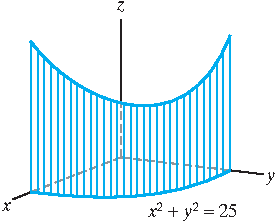
\includegraphics{img/6_1_34}
			\renewcommand{\thefigure}{6.16}
			\captionof{figure}{
				The picket fence of Exercise 34.
				The base of the fence is the quarter circle
				$x^2 + y^2 = 25$, $x,y \geq 0$.}
		\end{center}
	\end{problem}
	\begin{solution}
		
	\end{solution}
	
	\begin{problem}[6.1.40]
		You are traveling through Cleveland, 
		famous for its lake-effect snow in winter that makes driving quite treacherous. 
		Suppose that you are currently located 20 miles due east of Cleveland and 
		are attempting to drive to a point 20 miles due west of Cleveland. 
		Further suppose that if you are s miles from the center of Cleveland, 
		where the weather is the worst, you can drive at a rate of at most 
		$v(s) = 2s + 20$ miles per hour.
		\begin{subproblems}
			\subproblem
				How long will the trip take if you drive on a straight-line path directly through Cleveland?
				(Assume that you always drive at the maximum speed possible.)
				\begin{solution}
					
				\end{solution}
			\subproblem
				How long will the trip take if you avoid the middle of the city by driving along a
				semicircular path with Cleveland at the center? 
				(Again, assume that you drive at the maximum speed possible.)
				\begin{solution}
					
				\end{solution}
			\subproblem
				Repeat parts (a) and (b), this time using $v(s) = \frac{s^2}{16} + 25$ miles per hour 
				as the maximum speed that you can drive.
				\begin{solution}
					
				\end{solution}
		\end{subproblems}
	\end{problem}
\end{document}